\part{Speed Optimisation for Bitcoin Brain Wallet Attacks} \label{Part3}


\chapter{Improving Brain Wallet Attacks}
In Chapter \ref{Ch:EllipticCurve} we described the general concept of Ellipitic Curve and Bitcoin brain walltes. Brain wallets is a deterministic method to generate Bitcoin private keys from a password. This means once an attacker knows the password, they can recover the pravite key and get control of the Bitcoins within the wallet. Brain wallets exist because Bitcoin users prefer  to rememeber a password instead of keeping a long random string in a safe place. However, existing research discussed in Section \ref{sec:brainwalletRelatedWork} shows an attacker can simpely use a dictionary attack to guess the passwords. The security of Bitcoin Brain wallets only depends on the strength of the password. The  speed of checking if a guessed password leads to a used brain wallet only depends on the key generation process in the Bitcoin elliptic curve secp256k1. In this chapter we will review the current implementation of Bitcoin elliptic curve and provide detailed benchmarks on each elliptic curve opteration during the key geneartion process. At the end we will implement a new attack in order to speed up the key geneartion process and improve the existing attack.
\section{Bitcoin Elliptic Curve Implementation and Benchmarking}
\subsection{Dedicated Scalar Multiplication Method} \label {sec:specialMethod}
The process of cracking Bitcoin brain wallets is to repeatedly generated public keys using guessed passwords. The key generation method as we described in \ref{secKeyPairGen}, is to compute $Q = dP$. Here $d$ is a SHA256 hash of the generated password, $P$ is a fixed point which is the base point $G$ for secp256k1 (see Section \ref{sec:seckp256k1}). We first benchmark the current best implementation secp256k1 library. All benchmark results are running on a Intel i7-3520m 2.9GHz laptop (win8 x64).

The time cost for computing one public key given a random private key takes 
$$\textbf{47.2 us}. $$
\subsubsection{Fixed Point Multiplication Methods}
The most basic and naive method for point multiplication $Q=kP$ with a unknown point $P$ is the double-and-add method \cite{hankerson2006guide}.  The idea is to use binary representation for $k$:
$$ k = k_0 + 2k_1 + 2^2k_2+\cdots+2^mk_m$$
where $[k_0\dots k_m]\in \left\lbrace 0,1 \right\rbrace  $ and $m$ is the length of $k$, in Bitcoin elliptic curve, $m = 256$. 

 \begin{algorithm}[H] 
 	\caption{Double-and-add method for point multiplication of unknown points \cite{hankerson2006guide} page 96}
 	\label{alg:double-and-add}
 	INPUT: $k = (k_{m},...,k_1,k_0)_2$, $P \in E(\mathbb{F}_q)$. \\
 	OUTPUT: $kP$.
 	\begin{algorithmic} [1]
 		\STATE $Q := $ infinity
 		\FOR {$i$ from 0 to $m$} 
 		\STATE if $k_i$ = 1 then $Q := Q+P$  (using point addition)
 		\STATE $P:= 2P$ (using point doubling)
 		\ENDFOR
 		\RETURN $Q$
 	\end{algorithmic}
 \end{algorithm}

The expected number of ones in the binary representation of $k$ is approximately $\frac{m}{2}$, so the double-and-add method will need $\frac{m}{2}A + mD$ computations (where A means point addition and D means point doubling) in total. However, if the point $P$ is fixed and some storage is available, then the point multiplication operation $Q=kP$ can be accelerated by pre-computing some data that depends only on $P$. For example if the points $2P, 2^2P, \dots, 2^{m-1}P$ are precomputed, then the double-and-add method (Algorithm \ref{alg:double-and-add}) has an expected running time of $(\frac{m}{2})A$, and all doublings are eliminated.

In 1993, Brickell et al introduced a new method for fixed point multiplication \cite{brickell1993fast} . The precomputing step stores every multiple $2^iP$. Let $(K_{d-1},\dots,K_1,K_0)_{2^w}$ be the base-$2^w$ representation of $k$, where $d = [m/w]$, and let $Q_j = \sum_{i:K_i=j}2^{wi}P$ for each j, $1 \leq j \leq 2^w-1$, Then 
\begin{small}
\begin{multline} 
kP = \sum_{i=0}^{d_1}K_i(2^{wi}P) = \sum_{j=1}^{2^w-1}(j\sum_{i:K_i=j}2^{wi}P = \sum_{j=1}^{2^w-1}jQ_j\\
= Q_{2^w-1}+(Q_{2^w-1}+Q_{2^w-2})+\cdots+(Q_{2^w-1}+Q_{2^w-2}+\cdots+Q_1)
\end{multline}
\end{small}

\begin{algorithm}[h!] 
	\caption{Fixed-base windowing method for point multiplication\cite{hankerson2006guide}}
	\label{alg:fixed-baseWindow}
	INPUT: Window width $w$, $d = [m/w]$, $k=(K_{d-1},\dots,K_1,K_0)_{2^w}$\\
	OUTPUT: $kP$
	\begin{algorithmic} [1]
		\STATE Precompute $P_i = 2^{wi}P, 0 \leq i \leq d-1$
		\STATE $A \leftarrow \text{infinity}$, $B \leftarrow \text{infinity}$
		\FOR {$j$ from $2^w-1$ down to $1$} 
		\STATE For each $i$ for which $K_i = j$ do: $B \leftarrow B + P_i$
		\STATE $A \leftarrow A+B$
		\ENDFOR
		\RETURN $A$
	\end{algorithmic}
\end{algorithm}

Algorithm \ref{alg:fixed-baseWindow} has expected running time of  $$(2^w+d-3)A.$$
By reviewing the literature and checking some other existing methods in Hankerson's book \cite{hankerson2006guide} we noticed they are all memory friendly implementations which do not take a lot of memory for precomputation. However, we are working on a different task and aim at repeatedly running point multiplication method for great many times. We have implemented an extreme version of the window method which will take much more precomputation space than methods introduced by Hankerson \cite{hankerson2006guide}. 

In our implementation, the precomputation step will compute $P_j=jP$ where $ 1 \leq j \leq 2^w-1$ then for each $P_j$ we compute $P_{i,j}=2^{wi}P_j$, which will cost $2^w-1$ times more memory space than algorithm \ref{alg:fixed-baseWindow}, but expected running time for each point multiplication will reduce to approximately $(d-1)A$

\begin{algorithm}[H] 
	\caption{Our implementation of windowing method with larger precomputation table}
	\label{alg:newWindow}
	INPUT: Window width $w$, $d = [m/w]$, $k=(K_{d-1},\dots,K_1,K_0)_{2^w}$\\
	OUTPUT: $kP$
	\begin{algorithmic} [1]
		\STATE Precompute $P_{i,j} = 2^{wi}jP, 0 \leq i \leq d-1$ and $ 1 \leq j \leq 2^w-1$
		\STATE $A \leftarrow \text{infinity}$
		\FOR {$i$ from $0$ to $d-1$} 
		\STATE $A \leftarrow A+P_{i,j}$ where $j = K_i$
		\ENDFOR
		\RETURN $A$
	\end{algorithmic}
\end{algorithm}

We have implemented a code that can take any window width $w$ from 1 to 24\footnote{larger than 22 will take too long for precomputation and my laptop start to have slow response}, our benchmark results are shown in Table \ref{tb:benchmarkWindowSize1}. Note that precomputation stores elliptic curve point $P = {x,y}$ where $x$ and $y$ are 32 bits integer array of size 10. So one stored point needs 80 Bytes memory space. 
%\footnote{it will take a long time for my laptop to do precomputation when $w \gt 28$}

\begin{table}[h]
	\centering
	\caption{Time cost for different window width $w$, point addition method secp256k1 library \cite{Wulliesecp256k1} secp256k1\_gej\_add\_ge }
	\label{tb:benchmarkWindowSize1}
	\begin{tabular}{|c|c|c|c|c|c|}
		\hline
		& w=4 & w=8 & w=12 & w=16 & w=20 \\ \hline
		d         & 64  & 32  &  22  & 16   &   13   \\ \hline
		number of additions & 63 & 31 & 21 & 15 & 12 \\ \hline
		precomputation memory & 81.92 KB & 655.36 KB & 7.21 MB & 83.89 MB & 1.09 GB \\ \hline 
		time cost &  46.36 us & 22.76 us  &  15.35 us & 11.23 us &  9.23 us \\ \hline
	\end{tabular}
\end{table}
\subsection{Point Representation} \label{sec:pointRep}
As we described in Section \ref{sec:affine_formulas}, representing a point in affine coordinate $P(x,y)$ on an elliptic curve over $\mathbb{F}_p$, the field operations for calculating point addition needs 2 multiplications, 1 square and one modular inverse (for short, 2M+1S+1I). Modular inverse is a more expensive operation compared to multiplication and square. We list our benchmarks using different package in C to demonstrate the difference for modular inverse computation compare to multiplication and square. The packages we have benchmarked are: OpenSSL-1.0.2a (released in March 2015) and mpir-2.5.2 (released in Oct 2012), and the Pieter Wuille's implementation on github \cite{Wulliesecp256k1} \footnote{with the following configuration: USE\_NUM\_GMP USE\_FIELD\_10x26 USE\_FIELD\_INV\_NUM USE\_SCALAR\_8x32 USE\_SCALAR\_INV\_BUILTIN} . 


 The results are shown in Table \ref{table:benchmark_msi_affine}. The benchmarking shows modular inverse is much more expensive than multiplication and square. It is also important to notice, for OpenSSL Big Number library, a square operation is more expensive than multiplication, and for MPIR library, 1 square = 0.75 multiplication. As modular inverse is more expensive than multiplication, it may be advantageous to represent points using other coordinates.
 
 \begin{table}[]
 	\centering
 	\caption{Benchmarking OpenSSL and MPIR library for field multiplication, square and modular inverse in affine coordinate}
 	\label{table:benchmark_msi_affine}
 	\begin{tabular}{|c|c|c|c|c|c|}
 		\hline
 		& multiplication     & mod p    & square         & mod p        & mod inverse \\ \hline
 		MPIR      & 0.07 us            & 0.15 us    & 0.13 us        & 0.15 us        & 18.0 us     \\ \hline
 		OpenSSL   & 0.08 us            & 0.43 us    & 0.06 us        & 0.43 us        & 1.8 us      \\ \hline
 		secp256k1 & \multicolumn{2}{c|}{0.049 us} & \multicolumn{2}{c|}{0.039 us} & 1.1 us      \\ \hline
 	\end{tabular}
 \end{table}

\paragraph{Projective Coordinates} \mbox{}\\
For elliptic curve over $\mathbb{F}_p$ where the curve equation is $y^2=x^3+ax+b$. The standard projective coordinates represent elliptic curve points as ($X:Y:Z$), $Z \neq 0$, correspond to the affine point ($\frac{X}{Z},\frac{Y}{Z})$. The projective equation of the elliptic curve is: $$Y^2Z=X^3+aXZ^2+bZ^3$$ The point at infinity $O$ corresponds to (0:1:0), where the negative of ($X:Y:Z$) is $(X:-Y:Z)$ 
\paragraph{Jacobian Coordinates} \mbox{}\\
Elliptic curve points in Jacobian coordinate are represented in the following format ($X:Y:Z$), $Z \neq 0$, corresponds to the affine point $(\frac{X}{Z^2},\frac{X}{Z^3})$. The projective equation of the elliptic curve is $$ Y^2=X^3+aXZ^4+bZ^6$$ The point at infinity $O$ corresponds to (1:1:0), while the negative of ($X:Y:Z$) is ($X:-Y:Z)$.
 
The field operations needed for point addition and point doubling are shown in Table \ref{tb:APJacobian}. We see that Jacobian coordinates yield the fastest point doubling, while mixed Jacobian-affine coordinates yield the fastest point addition.

\begin{table}[h]
	\centering
	\caption{Operation counts for point addition and doubling. A = affine, P = standard projective, J = Jacobian \cite{hankerson2006guide,brown2001software}}
	\label{tb:APJacobian}
	\begin{tabular}{|cc|cc|ll|}
		\hline
		\multicolumn{2}{|c|}{Doubling} & \multicolumn{2}{c|}{General addition} & \multicolumn{2}{c|}{Mixed coordinates*} \\ \hline
		2A $\rightarrow$ A         & 1I,2M,2S        & A+A $\rightarrow$ A            & 1I,2M,1S           & \multicolumn{1}{c}{J+A $\rightarrow$ J}    & 8M,3S   \\
		2P $\rightarrow$ P         & 7M,3S           & P+P $\rightarrow$ P            & 12M,2S             &                              &         \\
		2J $\rightarrow$ J         & 4M,4S           & J+J $\rightarrow$ J            & 12M,4S             &                              &         \\ \hline
	\end{tabular} \par
	\bigskip
	* Here mixed coordinates means Jacobian-Affine mixed coordinates, see below for details.
\end{table}

We refer the reader to \cite{hankerson2006guide,brown2001software} for other detailed equations in different coordinates. Here we are only interested in point addition functions using mixed coordinates. 

\paragraph{Point Addition using Jacobian-Affine Mixed Coordinates} \mbox{} \\
Let $P = (X_1:Y_1:Z_1)$ be a Jacobian projective point on elliptic curve $y^2=x^3+ax+b$, and $Q = (X_2:Y_2:1)$ be be another point on the curve, suppose that $P \neq \pm Q$, $P+Q=(X_3:Y_3:Z_3)$ is computed by the following equations:
\begin{equation} \label{eq:8m3s}
\begin{split}
X_3 = &(Y_2Z_1^3-Y_1)^2 - (X_2Z_1^2-X_1)^2(X_1+X_2Z_1^2) \\
Y_3 = &(Y_2Z_1^3-Y_1)(X_1(X_2Z_1^2-X_1)^2-X_3)-Y_1(X_2Z_1^2-X_1)^3 \\
Z_3 = &(X_2Z_1^2-X_1)Z_1 
\end{split}
\end{equation}

By storing the intermediate elements, $X_3,Y_3$ and $Z_3$ can be computed using three field squarings and eight field multiplications as follows:

\begin{small}
$$ A \leftarrow Z_1^2, \text{ } B \leftarrow Z_1 \cdot A,  \text{ } C \leftarrow X_2 \cdot A,  \text{ } D \leftarrow Y_2 \cdot B,  \text{ }  E \leftarrow C - X_1,$$
$$ F \leftarrow D - Y_1, \text{ } G \leftarrow E^2, \text{ } H \leftarrow G \cdot E, \text{ } I \leftarrow X_1 \cdot G, $$
$$ X_3 \leftarrow F^2 - (H+2I), \text{ } Y_3 \leftarrow F \cdot (I - X_3) - Y_1 \cdot H, \text{ } Z_3 \leftarrow Z_1 \cdot E.$$
\end{small}
%In \cite{bernstein2007explicit} 

\paragraph{secp256k1 point addition formulas}
In the latest version, secp256k1 point addition formulas are based on Brier and Joye's work \cite{brier2002weierstrass} which introduced a strongly unified addition formulas for standard projective coordinate. Bitcoin developers implemented mixed coordinate formula (Jacobian-Affine) version based on Brier and Joye's work \cite{brier2002weierstrass}. 

Let $P = (X_1:Y_1:Z_1)$ be a Jacobian projective point on elliptic curve $y^2=x^3+ax+b$, and $Q = (X_2:Y_2:1)$ be be another point on the curve, suppose that $P \neq \pm Q$, $P+Q=(X_3:Y_3:Z_3)$ is computed by the following equations:
\begin{small}
\begin{equation} \label{eq:7m5s}
\begin{split}
X_3 &= 4 (K^2 - H) \\
Y_3 &= 4 (R(3H-2K^2)-G^2) \\
Z_3 &= 2 F  Z_1
\end{split}
\end{equation}
\end{small}
where
\begin{small}
$$ A = Z_1^2, \text{ } B = Z_1 \cdot A, \text{ } C = X_2 \cdot A, \text{ } D = Y_2 \cdot B, \text{ } E = X_1 + C $$
$$ F = Y_1 + D, G = F^2, H = E  \cdot G, I = E^2, J = X_1 \cdot C, K = I - J $$
\end{small}
\paragraph{Bernstein-Lange point addition formulas}
In \cite{bernstein2007faster}, Bernstein introduced the following method which takes 7M+4S; the explicit formulas are given as following \cite{bernstein2007explicit}
\begin{small}
\begin{equation} \label{eq:7m4s}
\begin{split}
& X_3 = r^2 - J - 2 V \\
& Y_3 = r \cdot (V-X_3)-2Y_1 \cdot J \\
& Z_3 = (Z_1+H)^2 - Z_1^2 - H^2 \\
\end{split}
\end{equation}
\text{where}\\
\begin{equation*}
\begin{split}
& U2 = X_2 \cdot Z_1^2,\text{ } S2 = Y_2 \cdot Z_1^3 \\
& H = U2 - X_1 , \text{ } I = 4 H^2 \\
& J = H \cdot I , \text{ } r = 2  (S2-Y_1) , \text{ } V = X_1 \cdot I 
\end{split}
\end{equation*}
\end{small}



\paragraph{Detailed Filed Operation Benchmarks} \mbox{} \\
From the results of Table \ref {table:benchmark_msi_affine} we saw that Wuille's secp256k1 library \cite{Wulliesecp256k1} has a much faster field multiplication and square speed than OpenSSL and mpir library.
Wuille's field implementation is optimised based on the prime used in secp256k1 curve. Secp256k1 library has 5x52 and 10x26 field implementation for 64 bits and 32 bits integers \footnote {Depends on whether compiler support 64 bits integer}. Here we use 10x26 representation and each 256 bits value is represented as a 32 bits integer array with size of 10. We refer readers to file \textit{field\_10x26\_impl.h} in secp256k1 library for more details. Secp256k1 library already implemented equation \ref{eq:7m5s} in method \textit{secp256k1\_gej\_add\_ge\_var}, which uses 8 multiplications, 3 squares and 12 multiply integer / addition / negation. Equation \ref{eq:8m3s} is implemented in \textit{secp256k1\_gej\_add\_ge} which uses 7 multiplications, 5 squares and 21 multiply integer / addition / negation. We have implemented equation \ref{eq:7m4s} which take 7 multiplication, 4 squares and 21 multiply integer / addition / negation.

It is important to notice the square and multiplication difference which we discussed in Table \ref{table:benchmark_msi_affine}. In \cite{explicitBernstein} Bernstein listed best operation counts based on different assumptions: S = 0M, S = 0.2M, S= 0.67M, S=0.8M and S=1M. Cohen discussed the ratio $S/M$ is almost independent of the field of definition and of the implementation, and can be reasonably taken to equal to 0.8 \cite{cohen1998efficient}. Our benchmark results are very similar to S = 0.8M (see Table \ref{table:benchmark_msi_affine}) . In Bernstein's work \cite{bernstein2007explicit}, other field operations are considered as 0M.  In Table \ref{tb:fieldoperationcounts} our benchmark results show field addition and other operations have approximately 0.1M cost. 

\begin{table}[h]
	\centering
	\caption{Field operation counts and benchmark results}
	\label{tb:fieldoperationcounts}
	\begin{tabular}{|c|c|c|c|c|c|}
		\hline
		& \#Mul & \#Square & \#add/neg/*int & \#fe\_cmov & total time cost    \\ 
	    & 1M & $\approx$ 0.8 M & $\approx$ 0.1 M  & $\approx$ 0.2 M  &    \\ \hline
		\begin{tabular}[c]{@{}l@{}}secp256k1\_gej\\ \_add\_ge\end{tabular}     & 7                & 5        & 15                 & 6        & $\approx$ 0.681 us \\ \hline
		\begin{tabular}[c]{@{}l@{}}secp256k1\_gej\\\_add\_ge\_var\end{tabular} & 8                & 3        & 12                 & 0        & $\approx$ 0.562 us \\ \hline
		7M + 4S  code    & 7                & 4        & 21                 & 0        & $\approx$ 0.594 us \\ \hline
	\end{tabular}
\end{table}

The secp256k1\_gej\_add\_ge method, which is also the default method for key generation, uses 6 secp256k1\_fe\_cmov operations which have a cost approximately 0.2 M. The main reason of writing code in such a way is stated in the code, and the author's comments: 
\begin{quotation}
\textit{"This formula has the benefit of being the same for both addition of distinct points and doubling"\cite{Wulliesecp256k1}}
\end{quotation}
The purpose of make addition and double using the same function is to prevent side channel attacks. As point doubling is much more cheaper than point addition. Our experiments are done based on the benchmark results of S/M ratio with specified machine setting (earlier in Section \ref{sec:specialMethod}) and a specific library configuration (footnote in Section \ref{sec:pointRep}). Different operating systems or library configurations might have different results. One should choose between our code and secp256k1\_gej\_add\_ge method. Detailed benchmark results are given in Table \ref{tb:benchmarkWindowSize}
% Our implementation method is chosen based on the benchmark results. One should chose the best method based on there square and multiplication performance. 

\begin{table}[h!]
	\centering
	\caption{Time cost for different window width $w$ for EC key generation}
	\label{tb:benchmarkWindowSize}
	\begin{tabular}{|c|c|c|c|c|c|}
		\hline
		& w=4                  & w=8       & w=12     & w=16     & w=20               \\ \hline
		d                                                                                                        & 64                   & 32        & 22       & 16       & 13                 \\ \hline
		 \# of additions                                                                                      & 63                   & 31        & 21       & 15       & 12                 \\ \hline
		\begin{tabular}[c]{@{}l@{}}precomputation\\ memory \end{tabular}                                                                                      & 81.92 KB             & 655.36 KB & 7.21 MB  & 83.89 MB & 1.09 GB            \\ \hline
		\begin{tabular}[c]{@{}l@{}}secp256k1\_gej\\ \_add\_ge\end{tabular}                                                                          & 45.85 us             & 22.16 us  & 15.35 us & 11.23 us & 9.23 us            \\ \hline
		\begin{tabular}[c]{@{}l@{}}secp256k1\_gej\\ \_add\_ge\_var\end{tabular}                                                                             & \textbf{37.37 us}* & 17.86 us  & 12.21 us & 8.89 us  & \textbf{7.16 us} \\ \hline
		7M + 4S code                                                                                             & 39.01 us             & 18.79 us  & 12.77 us & 9.23 us  & 7.48 us            \\ \hline
		\multicolumn{1}{|c|}{Jacobian to Affine}                                                          & \multicolumn{5}{c|}{  $\approx$ 10 us}                                               \\ \hline
		\multicolumn{1}{|c|}{\begin{tabular}[c]{@{}l@{}}Benchmark on  \\ my laptop \end{tabular}}      & \multicolumn{5}{c|}{\begin{tabular}[c]{@{}l@{}}$\approx$ 42 K guesses / sec (single thread)\\ on i7-3520m 2.9 GHz CPU\end{tabular}         }                                  \\ \hline
		DEF CON Attack**      & \multicolumn{5}{c|}{\begin{tabular}[c]{@{}l@{}}$\approx$ 130 K guesses / sec\\ on i7-2600 3.2 GHz CPU\end{tabular}                  }                                  \\ \hline
		\multicolumn{1}{|c|}{\begin{tabular}[c]{@{}l@{}}Improved \\ DEF CON Attack\end{tabular}                 }& \multicolumn{5}{c|}{ $\approx$ 315 K guesses / sec}                                  \\ \hline
	\end{tabular}
	\\ \mbox{} \\ * DEF CON attack \cite{RyanDefcon} is equivalent to this results 
	\\ ** Results are reported by Ryan Castellucci running his DEF CON code and our improved code on 8 threads with linux gcc compiler.
\end{table}

DEF CON attack \cite{RyanDefcon} published code on github in Aug using a faster version of secp256k1 library \footnote{Also written by Pieter Wuille one year ago, this version is performance focused and using 8M+3S}, and the results is marked as * in Table \ref{tb:benchmarkWindowSize}.  Our best result using 1.09 GB precomputation memory gives  \textbf{$\approx$ 2.5 times speed-up} for key generation process than the current known best attack.

Some work in this chapter has been developed into teaching materials for the UCL M.Sc. Information Security course, including low level c/c++ programming for field operation, ECDSA implementation and countermeasures against side channel attacks. 
\section{On Cracked Brain Wallets}
Our work has focused on providing the first detailed benchmark of existing Bitcoin elliptic curve implementations and optimizing the speed of the state-of-art Bitcoin brain wallets attack. We did not pay attention to analysing the cracked brain wallets. We refer the reader to read Vasek's paper \cite{vasek2016bitcoin} for a detailed measurement of cracked brain wallets results. In this section we only give a brief summary of our results and discuss some interesting points which are not covered by Vasek's research.

We have collected all hash160 on blockchain data (until June 2015). 89,872,723 unique addresses have ever been used, and we have cracked 18,350 addresses in total. All of them were empty at the time we found them. It is clear that the majority of addresses had been registered by a single entity (some sort of bounty or honeypot). 17784 brain wallets were first used on August 31, 2013 and have the same transaction amount 0.00005460 bitcoin or precisely twice this amount. The largest amount ever seen in one brain wallet was 500 BTC. 

\subsection{Network Stress Test}
The maximum block size of Bitcoin is one megabyte per block. On 11 November 2014, when the block was around 30\% full, David Hunduson wrote a blog post \cite{DavidHunduson2015} analyzing what will happen as the network approaches 100\% full. The author did a simulation which shows that if the block is 100\% full, then 10\% of all transactions would still not have received a confirmation after 22800 seconds (Bitcoin transcations are normally confirmed after around 600 seconds).
Later, on 4th May 2015, Gavin Andersen published his first in a series of blog posts \cite{Andersen2015} aimed at convincing the Bitcoin community to adopt a larger block size. This sparked a heated debate about the Bitcoin blocksize that broke past the technical developers of the Bitcoin protocol into the broader sphere of people that care about Bitcoin. As a result of this debate, several network stress tests were launched. We measured some aftermath of this contentious test, since the perpetrator / originator chose to send large quantities of small amounts of bitcoin to selected brain wallets. Between 28th June 2015 and 28th August  2015, we observed 41 addresses used in the network stress test (also known as ``July flood attack'') with a total number of 1,554,187 transactions and total amount of 46.8 BTC.  

\subsection{Disclosure of Results}
Although all the cracked brain wallets are currently empty, we still decided not to publish a full list of cracked passwords or Bitcoin addresses because users can make the same mistake again. Even statistical information about weak wallets helps attackers to steal more bitcoins. We have given some sample passwords in appendix \ref{appendixlabel2}. One possible way for disclosure is to tag the cracked addresses on blockchain.info. See Figure \ref{fig:tagged_address}. Bitcoin users can see if their brain wallet address is cracked. But the process is not automated due to captcha requirement and we do have a lot of cracked passwords.
 
  \begin{figure}[h!]
  	\centering
  	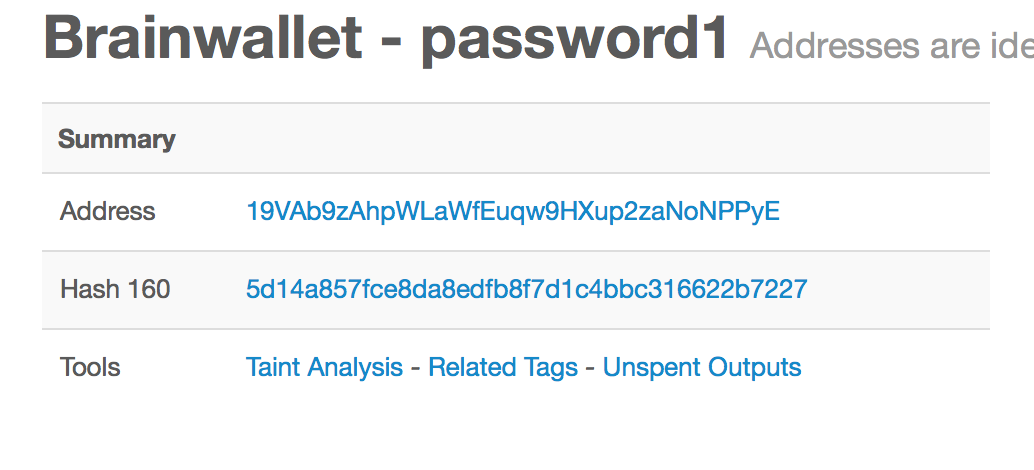
\includegraphics[width=100mm]{./pics/tag_address.png}
  	\caption{Example of tagged brain wallet address }
  	\label{fig:tagged_address}
  \end{figure}
  
\section{Summary}
In this chapter we have analysed and improved the state of the art on the implementation of the secp256k1 elliptic curve and similar curves. We provided the first benchmarks on existing implementations and provided a faster implementation for specific applications where private keys are not manipulated or there exist other protections against side channel attacks [e.g. physical and electro-magnetic isolation] and when larger amounts of RAM are available. We are able to examine passwords in brain wallets 2.5 times faster than the state of the art implementation presented at DEF CON. We have released our source code. As an example application of this research, we have been able to crack thousands of passwords including some quite difficult ones.

The idea behind Bitcoin brain wallets is elegant: remembering a password or passphrase is surely easier than a private key. Our work and also Vasek's work \cite{vasek2016bitcoin} have made a clear point that it is an extremely insecure way to store bitcoin. There exist lots of other methods to keep bitcoin more secure. As a result of our research, the first and widely suggested brain wallet generation website brainwallet.org has been permanently closed.  
